\section{Interaction}
\label{sect:exp}

We present here a grasping behavior based on the modules described in the previous sections. The interaction with the environment starts when an object is placed in the robot's hand; the robot detects the object by using the tactile sensors on the palm (see figure \ref{fig-experiment} frame 1). When pressure on the palm is detected the fingers close in a stereotyped grasping action. The intrinsic elasticity of the hand (see section \ref{sect:robot}) facilitates grasping, because the fingers automatically adapt to the shape of the object. The robot starts the exploration of the object by bringing it close to the cameras in four different positions and orientations (frames 2-3). During the exploration the robot keeps fixation on the object by tracking the hand. At each position a few frames are acquired and processed as explained in section \ref{sect:vision} to train the model of the object. As the exploration is completed the object is dropped on the table. The robot exploits now the visual model of the object to search for it again (meanwhile the object might have been moved elsewhere by the experimented) in the visual scene. 

The search procedure is driven by a top-down attention module whose contribution exploits the knowledge the robot just acquired about the object. In practice, this happens by selecting the blob whose features better match those of the object's main blob and performing a saccade motion towards it. After the saccade the object is in the fovea (frame 4 and 7) and its model is matched against the blobs that are now fixated. If the match is positive grasping starts otherwise search continues. The disparity map of the segmented object is computed to determine the orientation of the object (frames 5 and 8); two different actions are then attempted to maximize the possibility to successfully grasp the object. If the principal axis is oriented horizontally the robot moves the hand above the object, otherwise the hand approaches the object from the side (frames 6 and 9). To determine if the grasping is successful, the robot checks the weight of the object and its ``consistence'' in the hand (the shape of the fingers around the object). In case of failure another grasping trial is attempted, otherwise the robot waits for a new object to be placed in the palm.

\begin{figure}
\centering
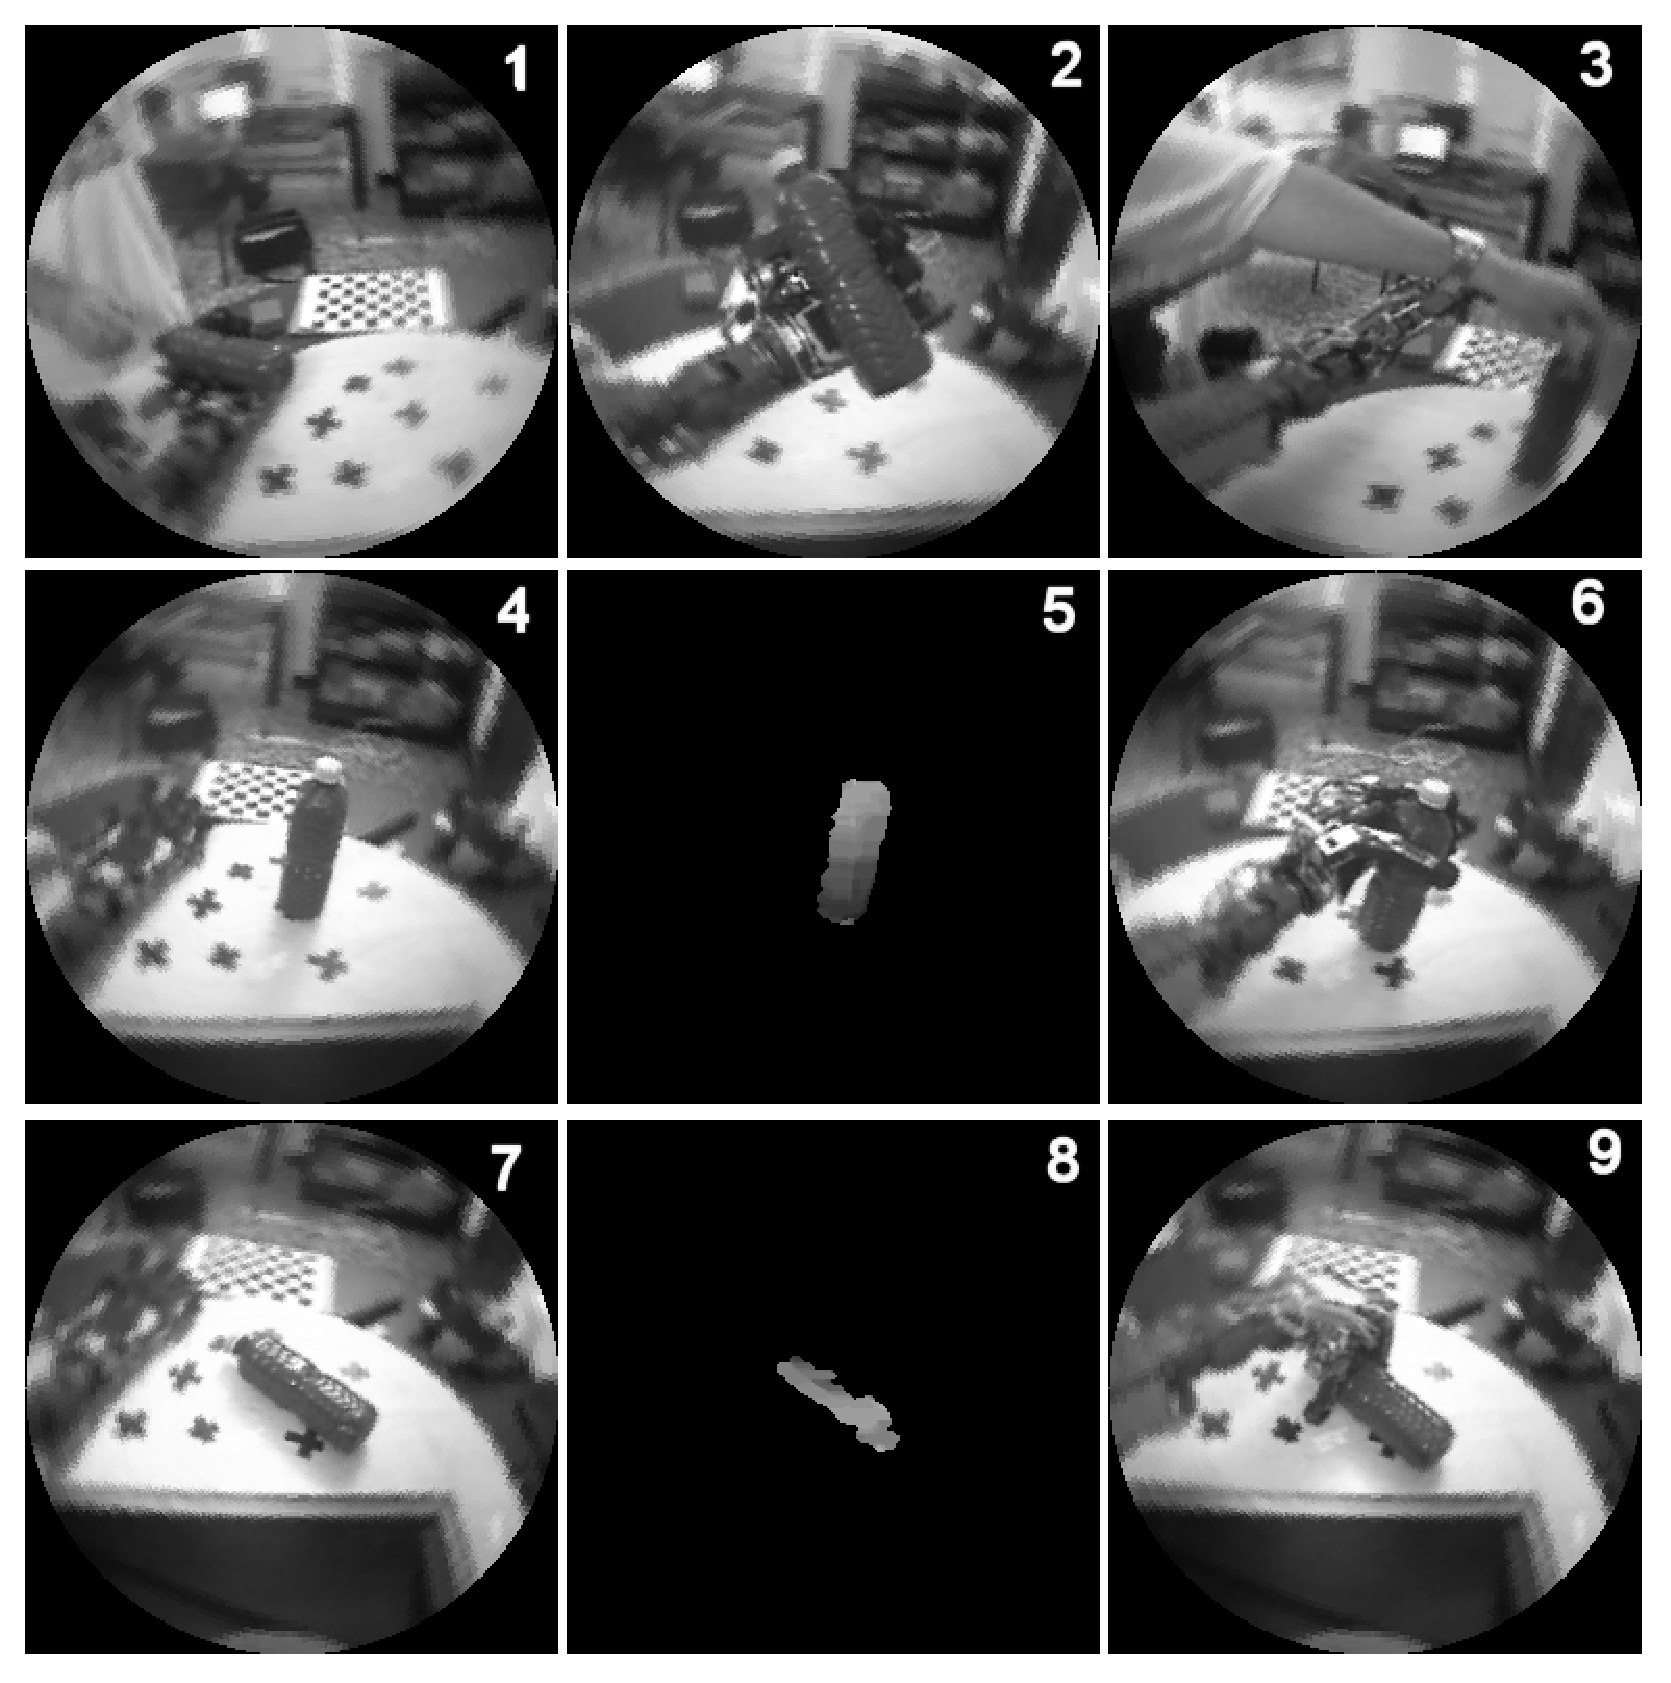
\includegraphics[width=3in]{experimental}
\caption{The execution of a grasping experiment.}
\label{fig-experiment}
\end{figure}
